\documentclass[11pt,a4paper]{article}
\usepackage[utf8]{inputenc}
\usepackage[german]{babel}
\usepackage[T1]{fontenc}
\usepackage{amsmath}
\usepackage{amsfonts}
\usepackage{amssymb}
\usepackage{graphicx}
\usepackage[margin=1.25cm]{geometry} % Puts the same margin on all borders of the document

% Packages

\usepackage{hyperref} % Generate hyperlinks to referenced items
\usepackage{adjustbox} % Used to change parameters in \includegraphics[scale=•]{•}
\usepackage{enumitem} % Provides several options for lists
\usepackage{verbatim} % Package to use \begin{comment}
\usepackage{pdfpages} % Used to import PDF pages
\usepackage{multirow} % Allows us to have a single cell in a table span multiple rows
\usepackage{makecell} % Allows us to format multiple lines in a single cell
\usepackage{minted} % Used to syntax highlight code
\usepackage{xcolor}  % Gives access to coloring text
\usepackage{longtable} % Allows us to create a table over multiple pages
\usepackage{float} % Improved placement of floating items
\usepackage{pdfpages} % Used to import pdf pages
\usepackage{booktabs} % Used for horizontal lines instead of \hline



% Settings

\graphicspath{{./files/}} % Sets path for files to the files folder in the same directory

\hypersetup{
    colorlinks=false, %set true if you want colored links
    linktoc=all,     %set to all if you want both sections and subsections linked
    linkcolor=blue,  %choose some color if you want links to stand out
}


\renewcommand{\arraystretch}{1.25} 

\begin{titlepage}
  \title{FOP Reference Sheet} % document_name-type_of_document
  \author{Jonas Milkovits}
  \date{Last Edited: \today}
\end{titlepage}

\begin{document}

\pagenumbering{gobble}
\maketitle
\pagenumbering{roman} % i, ii, iii on beginning pages, that don't have content
\tableofcontents
\clearpage
\pagenumbering{arabic} % 1,2,3 on content pages

\section{Computerspeicher}
\begin{itemize}
\item Unsere Vorstellung: großes Feld aus Maschinenwörtern mit eindeutiger Adresse

\item[] \begin{center}
		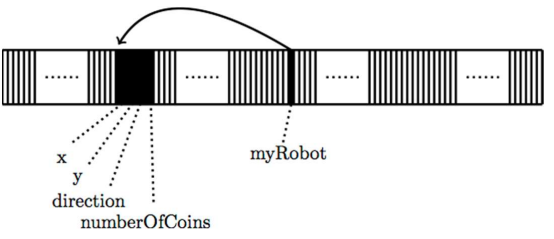
\includegraphics[scale=0.8]{computerspeicher}
		\end{center}

\end{itemize}

\section{Klassen und Methoden}

\begin{tabular}{ | p{4cm} p{11.5cm} p{1.5cm} | }
\hline
&&\\ \hline






\end{tabular}



\end{document}